\chapter{Аналитическая часть}

\section{Волновой процесс}

При каком-либо внешнем воздействии на поверхность воды (ветер, движение корабля, падение камня) частицы жидкости опускаются вниз, и водная поверхность становится вогнутой. Сила тяжести и/или сила поверхностного натяжения стремятся вернуть частицы в состояние равновесия. При этом частицы воды переходят это положение, и поверхность воды становится выпуклой. Движение передается от одних частиц к другим. Так на водной поверхности появляются волны. Волновой процесс показан на рисунке 1.1.

\begin{figure}[H]
	\begin{center}
		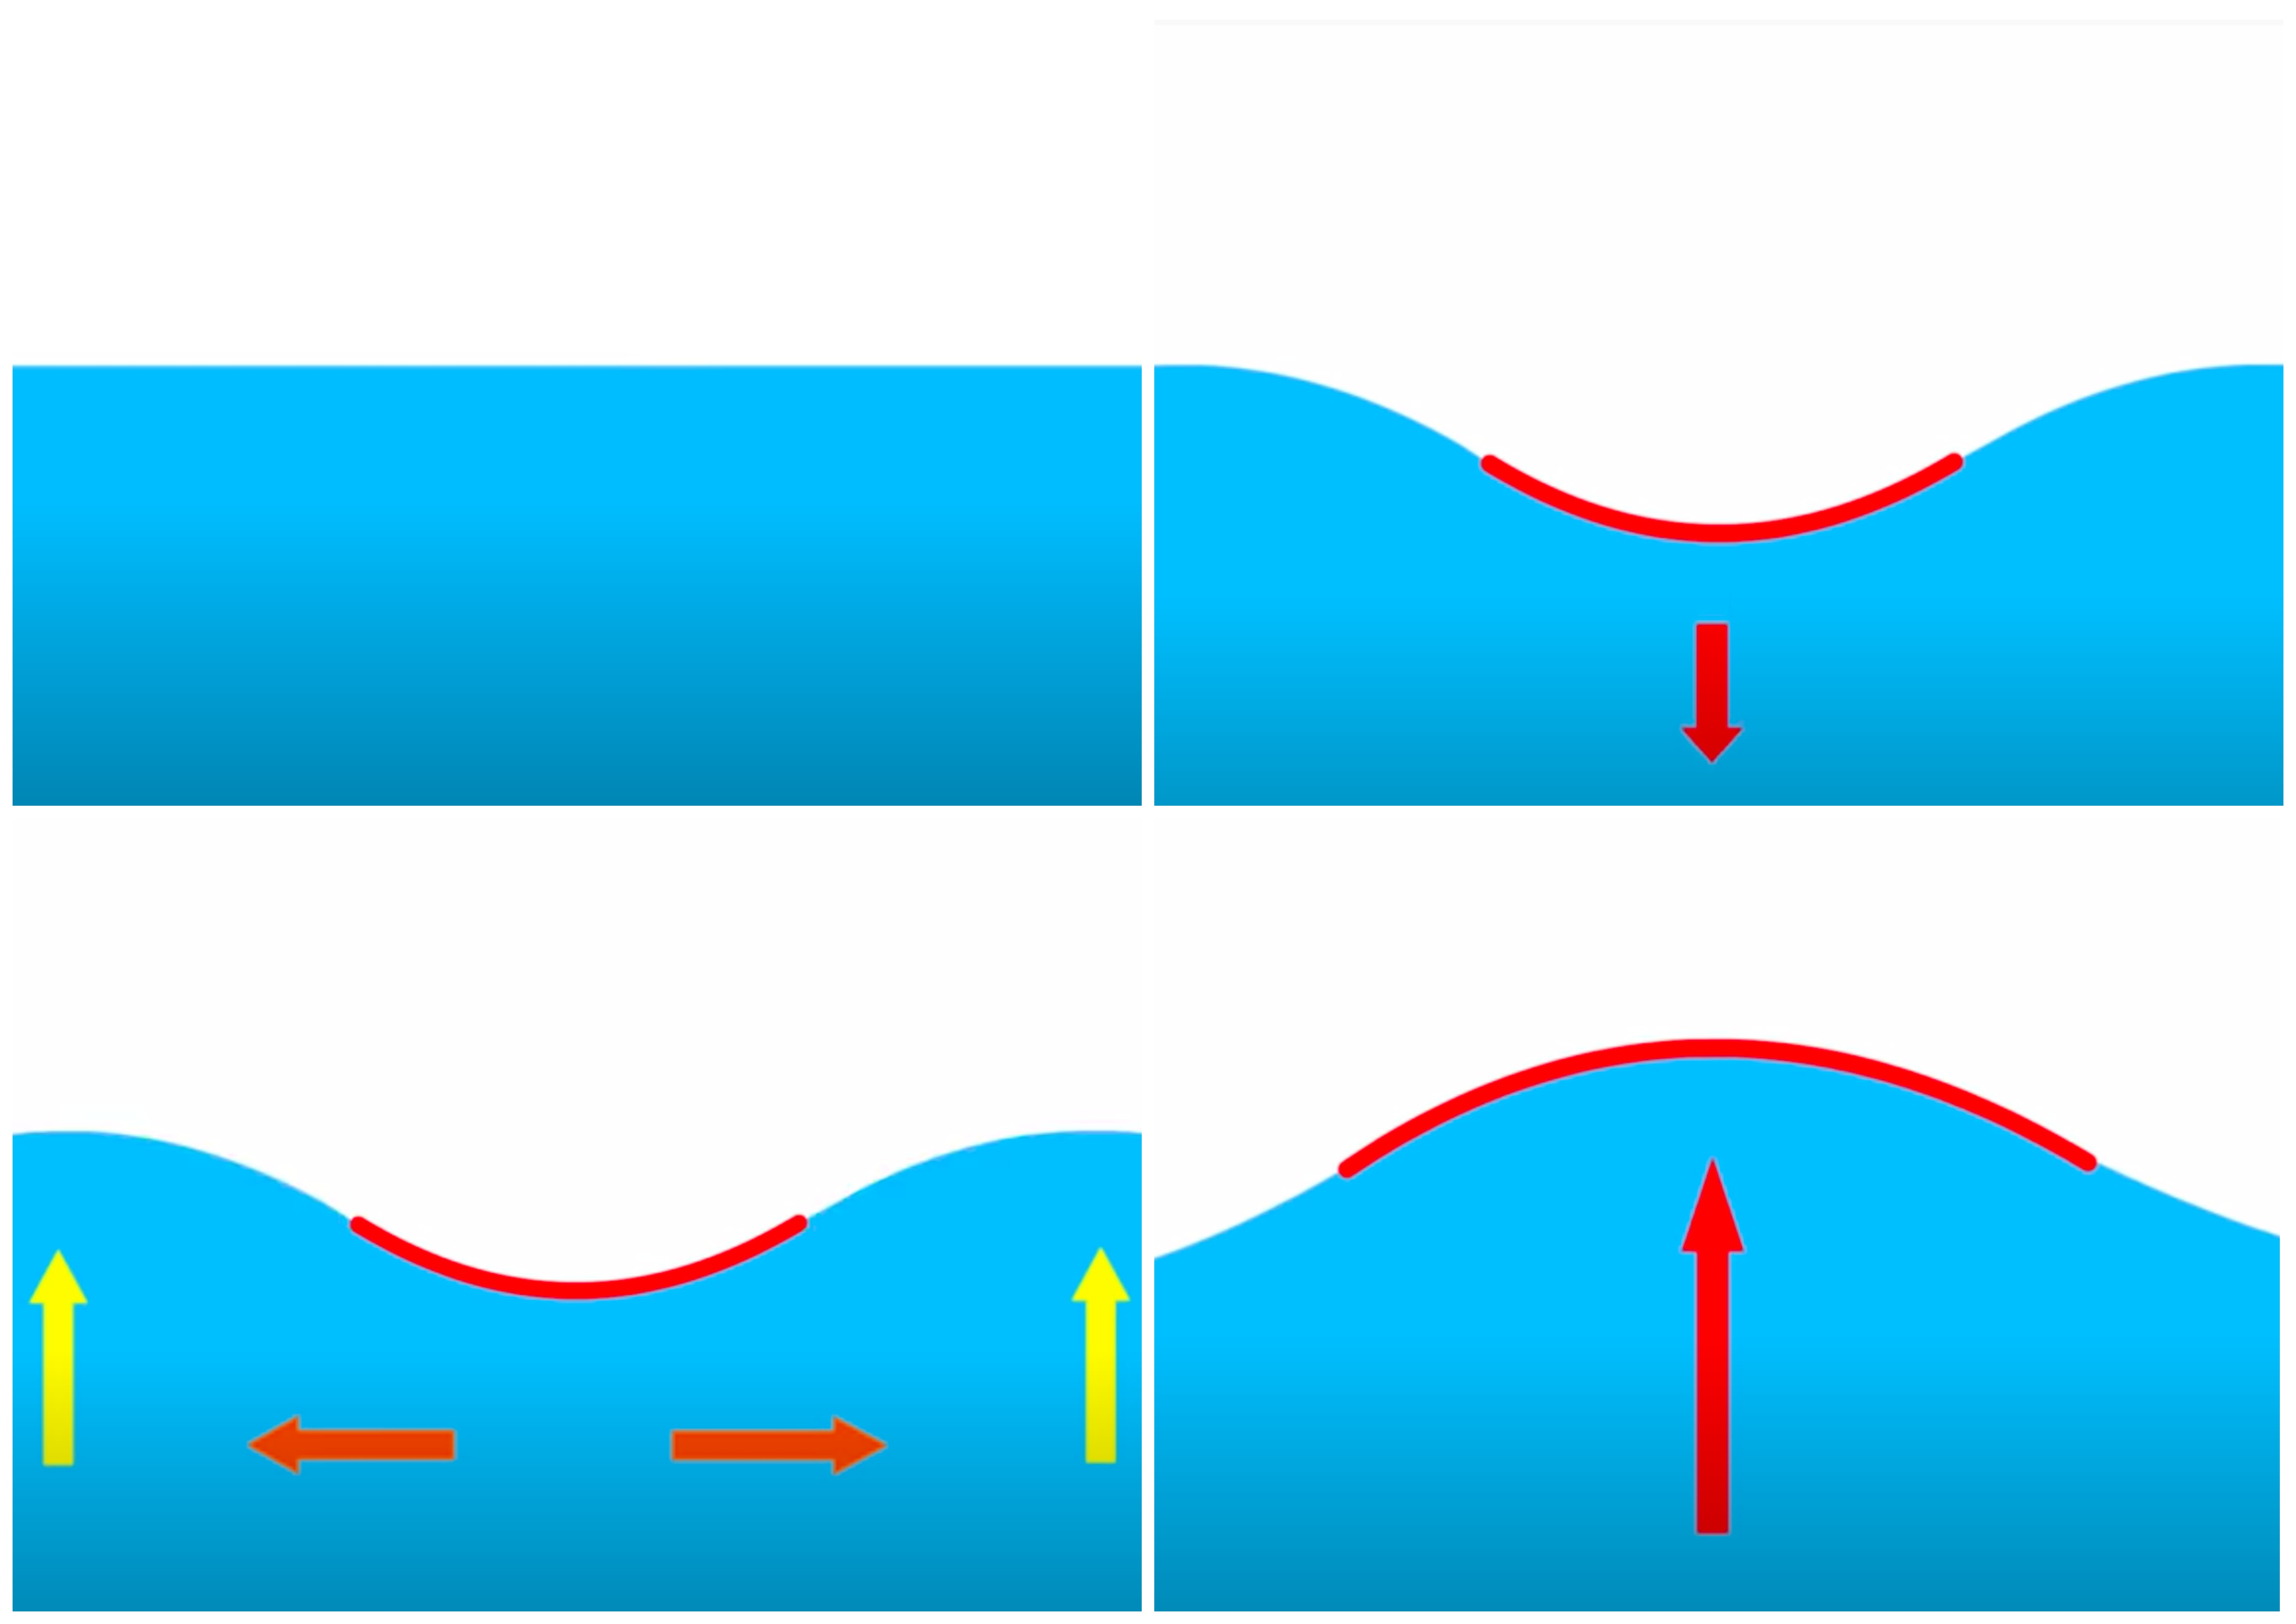
\includegraphics[scale=0.08]{img/wave-process.jpg}
	\end{center}
	\captionsetup{justification=centering}
	\caption{Процесс образования волны.}
	\label{img:wave-process}
\end{figure}

Если восстановить равновесие стремится сила тяжести, то волны называются гравитационными, если сила поверхностного натяжения - капиллярными. Когда силы сопоставимы, волны называют капиллярно-гравитационными. Механизм образования волн подчиняется закону дисперсии. Дисперсия волн - это зависимость скорости распространения волн от их частоты. Именно дисперсия создает сложную картину волн, образованных телом в воде.

В зависимости от требований к результату моделирования выбирается определенный метод визуализации. Так как в центре работы диспергирующие волны, для выполненения поставленных задач необходим такой метод моделирования, при котором выполняется дисперсионное соотношение, т. е. корректно обрабытывается взаимодействие волны и объекта.

\section{Методы визуализации волн}

Существует три группы методов моделирования волн:

\begin{itemize}
    \item процедурные;
    \item методы на основе частиц;
    \item методы поля высот.
\end{itemize}

\subsection{Процедурные методы}

В процедурных методах для представления движения волн используются периодические функции. В ранних работах в качестве такой функции выступала циклоида \cite{orbit-procedure}, далее стали использовать синусоиду \cite{spectrum-darles}. Наложение периодических функций, изменяющихся во времени, создает волновую поверхность. Точка на такой поверхности описывает замкнутую круговую орбиту. Для создания различных волновых эффектов изменяют параметры уравнений орбиты, например, радиус, фазовый угол.

Процедурные методы чаще всего используют при визуализации масштабных волн океана. Преимуществом процедурного моделирования является возможность точно контролировать движение волнового спектра. Недостаток данных методов - сложность получения правильного взаимодействия волн с погруженными телами и границами.  

Выделяют следующие процедурные методы:

\begin{itemize}
    \item метод, основанный на модели Герстнера;
    
Данный метод основан на решении уравнения Эйлера для гравитационных волн. Каждая частица на водной поверхности описывает окружность вокруг положения покоя. Тогда поверхность воды - кривая, которую описывает частица, находящаяся на расстоянии от центра окружности, которая катится по направляющей, как показано на рисунке 1.2. Эту кривую называют трохоидой. Используя лагранжевую систему отсчета находят все необходимые для визуализации параметры волн \cite{orbit-procedure}.

\begin{figure}[H]
	\begin{center}
		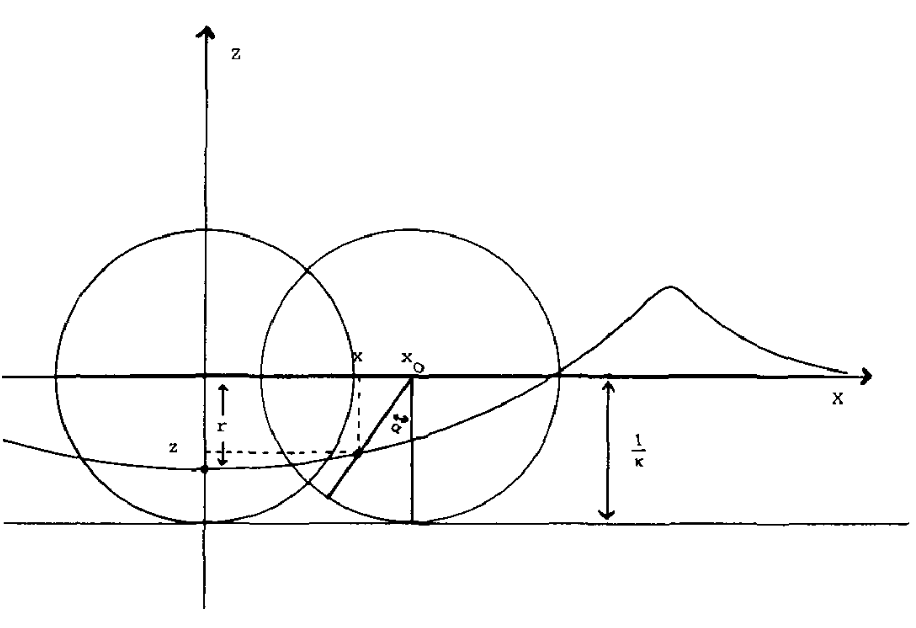
\includegraphics[scale=0.3]{img/trochoid.png}
	\end{center}
	\captionsetup{justification=centering}
	\caption{Поверхность воды представлена трохоидой.}
	\label{img:trochoid}
\end{figure}

    \item спектральные подходы. 

В данных подходах поверхность океана - поле высот, которое имеет спектр, соответствующий значениям реальной волновой поверхности. Генерируются синусоидальные волны, которые приближенно соответствуют реальным волнам. Если рассматривать функцию представления волны в частотной области, то можно добиться получения трохоид \cite{spectrum-darles}\cite{spectrum-tessendorf}.
\end{itemize}

\subsection{Методы на основе частиц}

В следующих методах моделирования волновой поверхности вода представляется как система частиц. Частицы движутся в соответствии с законами механики и обладают физическими величинами, т. е. задана функция. В определенный момент времени при помощи интерполяции можно получить значение этой функции в произвольной точке.

Для создания реалистичного изображения необходимо большое количество частиц, поэтому даннные методы используются при визуализации небольшого количества воды.  

Наиболее распространнёные методы на основе частиц:

\begin{itemize}
    \item гидродинамика сглаженных частиц (SPH) \cite{sph};
    \item полунеявный метод движущихся частив (MPS) \cite{mps}.
\end{itemize}

Комбинация методов полей высот и методов, основанных на частицах, позволяет обходить недостатки отдельных и создавать различные эффекты \cite{shallow}\cite{large-small}.

\subsection{Методы поля высот}

В случаях, когда визуализировать необходимо только поверхность воды,а не весь объем водоема, рассматривают волновое уравнение. Волновая поверхность представляется в виде двумерной функции - поля высот \cite{field}. 

Такое упрощение обладает важным преимуществом - снижением вычислительных затрат, что означает повышение скорости моделирования. Кроме того методы поля высот гибко обрабатывают препятствия. Но при такой модели в каждой точке поверхности известно только одно значение высоты, что означает одинаковую скорость распространения всех волн, так, невозможно создать обрушивающиеся волны.

\section{Модели волны и предмета}

\subsection{Модель волны}



\subsection{Модель предмета}

В центре рассматриваемой системы движения диспергирующих волн, которые образованы в результате контакта поверхности воды с предметом. Для правильной обработки отражения волн от твердых тел важны параметры только той части предмета, которая касается воды.  В связи с этим нет необходимости рассматривать объект детально. Поэтому для его представления требуется такой параметр, как площадь соприкосновения.

\section{Существующие программные обеспечения}

\section{Анализ алгоритмов удаления невидимых линий и поверхностей}

Сравню алгоритмы удаления невидимых линий и поверхностей по критериям. В выводе подраздела выберу лучший.

\section{Анализ методов закрашивания}

Сравню методы закрашивания по параметрам. В выводе подраздела выберу победителя.

\section{Модель освещения}

Опишу модели освещения. Выберу подходящую.

В конце подытожу все.